

\subsubsection{ Return paths}
In this section, we explain the gadgets used after a digit and its {\dtop} gadget have assembled. These
are the return paths, the purpose of these gadgets is to route the counter to the next place it needs to be, which
could be the next digit, a new row, etc.


For each $\inc\in \{ {\tt increment}, {\tt copy} \}$:

\begin{itemize}

    % DIGIT 1
    \item Create
    $\begin{aligned}[t]
        \returnpath(& \left\langle {\tt ReturnPath},    1, \inc \right\rangle,
                           \left\langle {\tt NextRead}, 1, \inc \right\rangle \;)
    \end{aligned}$\\from the micro-gadget shown in Figure~\ref{fig:return_path_1_op}.

    \item Create
    $\begin{aligned}[t]
        \returnpath(& \left\langle {\tt ReturnPath},    1, \inc, {\tt msr} \right\rangle,
                           \left\langle {\tt NextRead}, 1, \inc, {\tt msr} \right\rangle \;)
    \end{aligned}$\\from the micro-gadget shown in Figure~\ref{fig:return_path_1_op_msr}

    \item Create
    $\begin{aligned}[t]
        \returnpath(& \left\langle {\tt ReturnPath},    1, \inc, {\tt msr}, {\tt msd} \right\rangle,
                           \left\langle {\tt NextRead}, 1, \inc, {\tt msr}, {\tt msd} \right\rangle \;)
    \end{aligned}$\\from the micro-gadget shown in Figure~\ref{fig:return_path_1-or-2_op_msr_msd}.


    % DIGIT 2
    \item Create
    $\begin{aligned}[t]
        \returnpath(& \left\langle {\tt ReturnPath},    2, \inc \right\rangle,
                           \left\langle {\tt NextRead}, 2, \inc \right\rangle \;)
    \end{aligned}$\\from the micro-gadget shown in Figure~\ref{fig:return_path_2_op-or-seed}.

    \item Create
    $\begin{aligned}[t]
        \returnpath(& \left\langle {\tt ReturnPath},    2, \inc, {\tt msr}, {\tt msd} \right\rangle,
                           \left\langle {\tt NextRead}, 2, \inc, {\tt msr}, {\tt msd} \right\rangle \;)
    \end{aligned}$\\from the micro-gadget shown in Figure~\ref{fig:return_path_1-or-2_op_msr_msd}.



    % DIGIT 3
    \item Create
    $\begin{aligned}[t]
        \returnpath(& \left\langle {\tt ReturnPath},    3, \inc \right\rangle,
                           \left\langle {\tt NextRead}, 3, \inc \right\rangle \;)
    \end{aligned}$\\from the micro-gadget shown in Figure~\ref{fig:return_path_3}.


    \item Create
    $\begin{aligned}[t]
        \returnpath(& \left\langle {\tt ReturnPath},    3, \inc, {\tt msr}, {\tt msd} \right\rangle,
                           \left\langle {\tt NextRead}, 3, \inc, {\tt msr}, {\tt msd} \right\rangle \;)
    \end{aligned}$\\from the micro-gadget shown in Figure~\ref{fig:return_path_3}.

\end{itemize}

\begin{figure}[H]
    \centering
    \subcaptionbox{Digit 1 - general \label{fig:return_path_1_op}}
    {\makebox[0.24\textwidth][c]{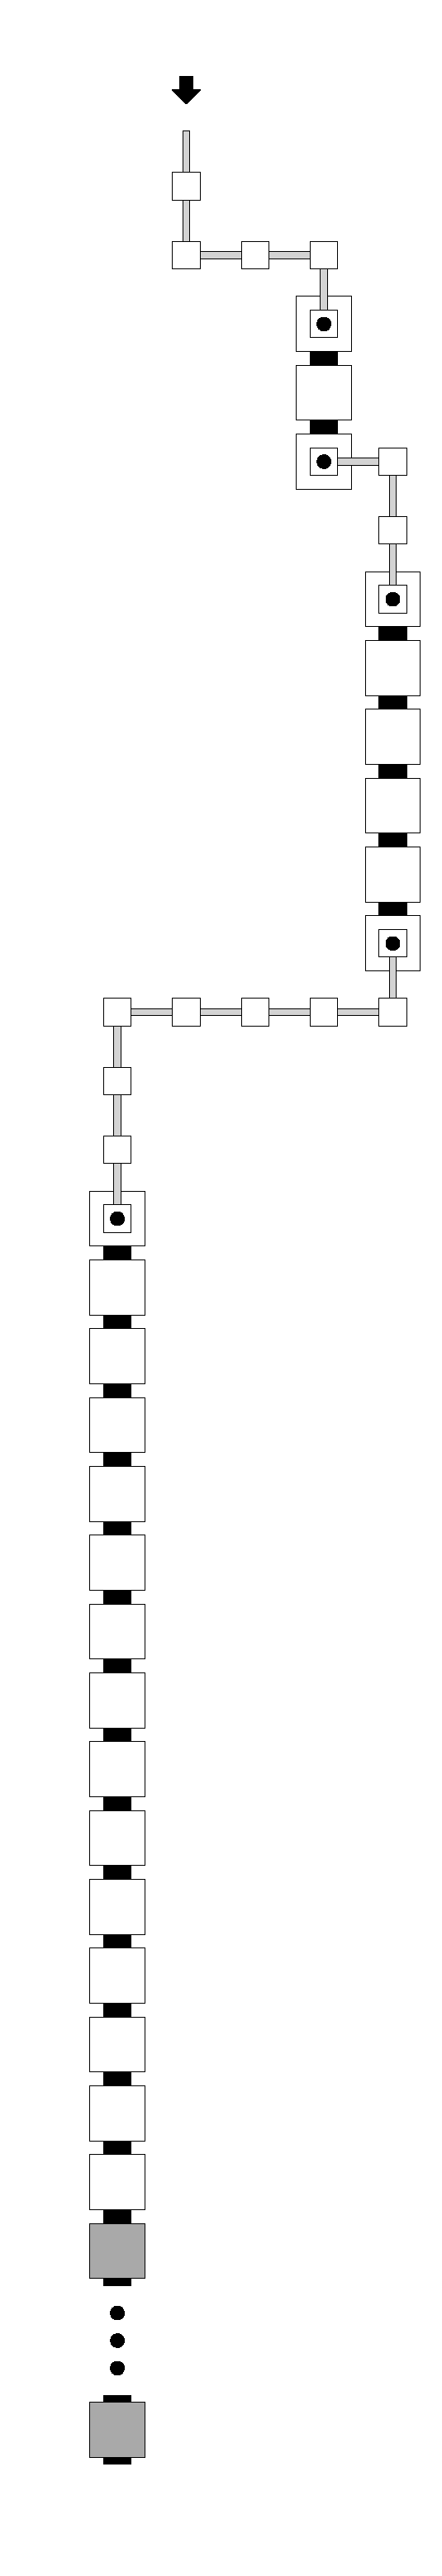
\includegraphics[width=0.45in]{return_path_1_op}}}%
    ~
    \subcaptionbox{Digit 1 - general\\overview\label{fig:return_path_1_op_overview}}
    {\makebox[0.24\textwidth][c]{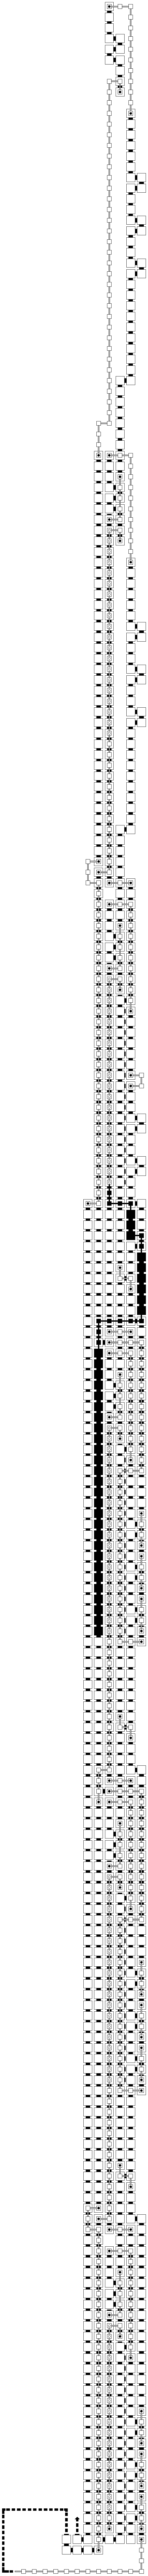
\includegraphics[width=0.45in]{overviews/general/return_path_1_op}}}%
    ~
    \subcaptionbox{Digit 1 - general (seed) overview\label{fig:return_path_1_seed_op_overview}}
    {\makebox[0.24\textwidth][c]{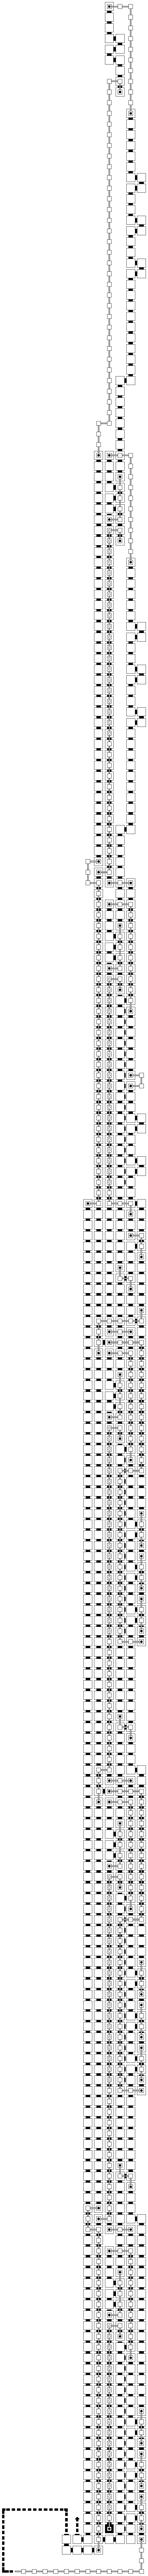
\includegraphics[width=0.45in]{overviews/general/return_path_1_seed_op}}}%
    ~
    \subcaptionbox{Digit 2 - general \label{fig:return_path_2_op-or-seed}}
    {\makebox[0.24\textwidth][c]{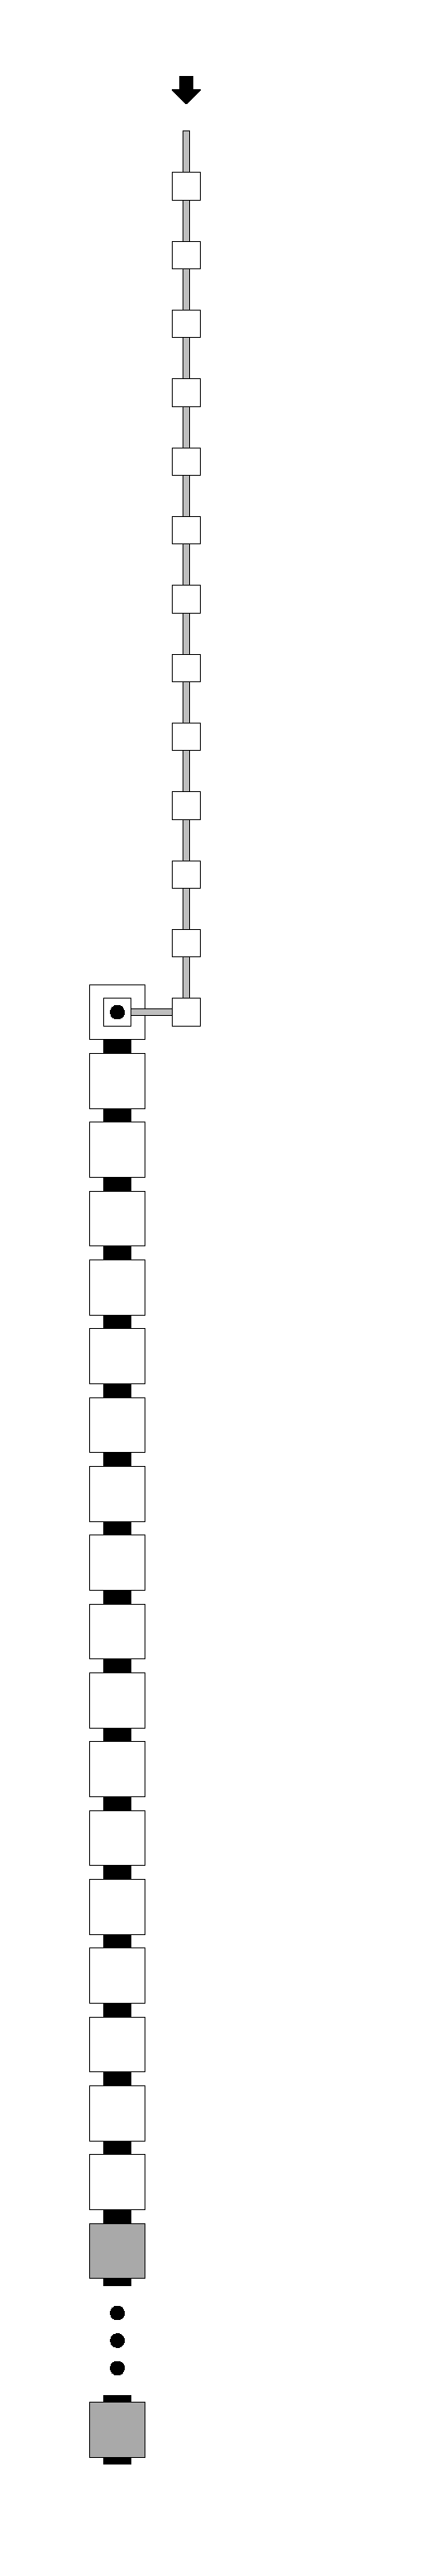
\includegraphics[width=0.45in]{return_path_2_op-or-seed}}}%
    ~
\end{figure}
\begin{figure}[H]\ContinuedFloat
    \centering
    \subcaptionbox{Digit 2 - general\\overview\label{fig:return_path_2_op_overview}}
    {\makebox[0.24\textwidth][c]{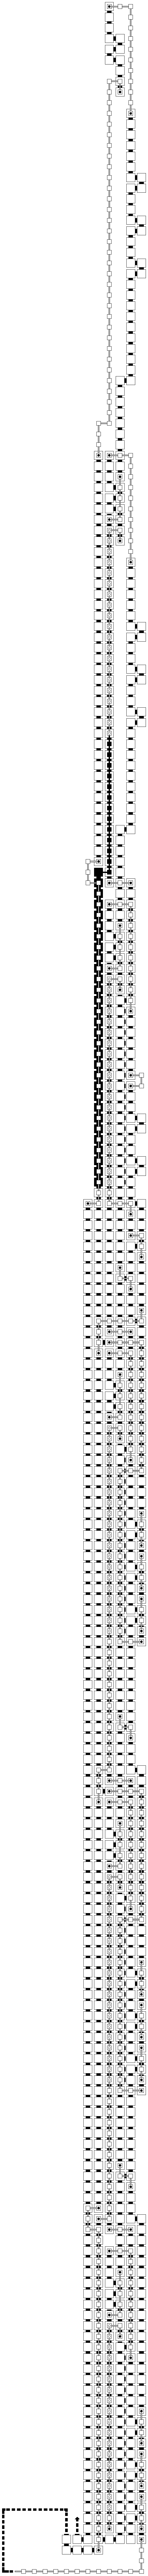
\includegraphics[width=0.45in]{overviews/general/return_path_2_op}}}%
    ~
    \subcaptionbox{Digit 2 - general (seed) overview\label{fig:return_path_2_seed_op_overview}}
    {\makebox[0.24\textwidth][c]{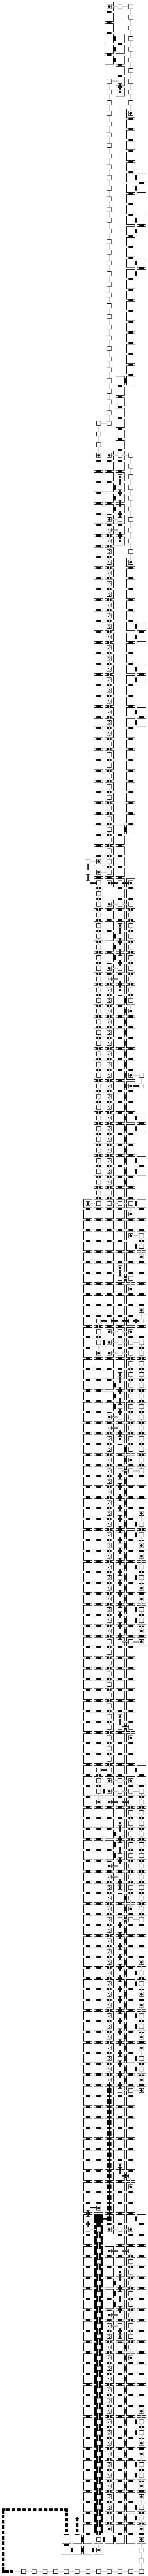
\includegraphics[width=0.45in]{overviews/general/return_path_2_seed_op}}}%
    ~
    \subcaptionbox{Digit 3 - general \label{fig:return_path_3}}
    {\makebox[0.24\textwidth][c]{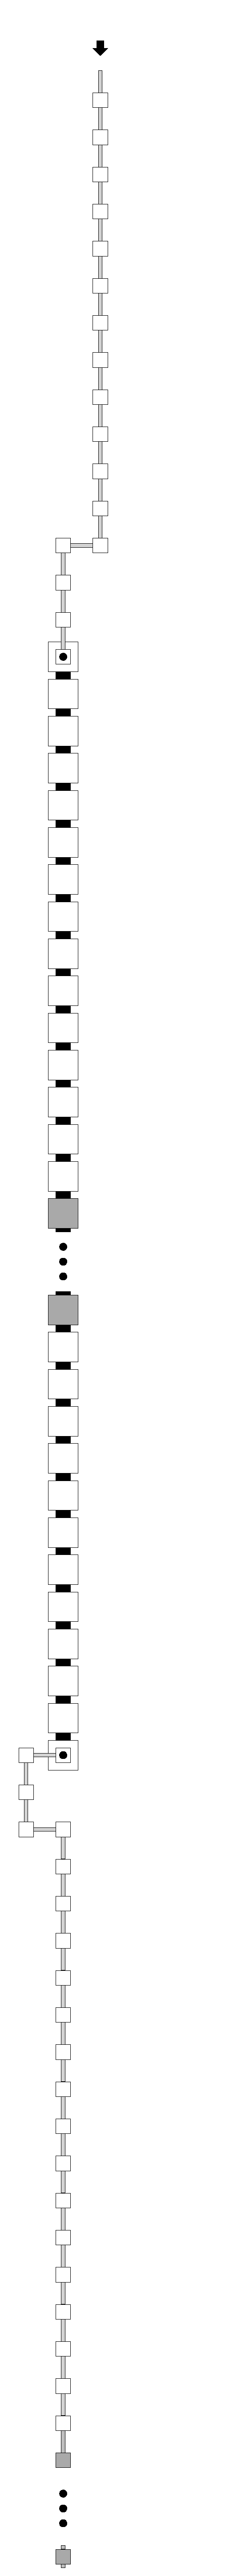
\includegraphics[width=0.45in]{return_path_3}}}%
    ~
    \subcaptionbox{Digit 3 - general\\overview\label{fig:return_path_3_op_overview}}
    {\makebox[0.24\textwidth][c]{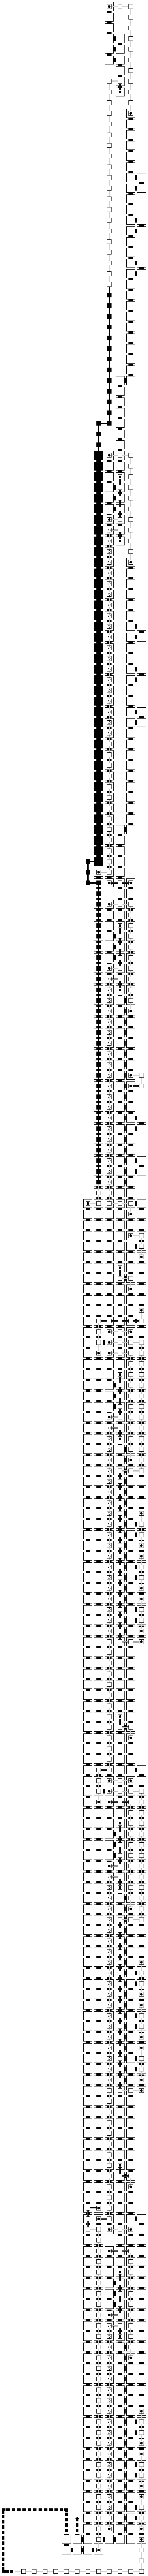
\includegraphics[width=0.45in]{overviews/general/return_path_3_op}}}%
    ~
\end{figure}

\begin{figure}[H]\ContinuedFloat
    \centering
    \subcaptionbox{Digit 3 - general (seed) overview\label{fig:return_path_3_seed_op_overview}}
    {\makebox[0.24\textwidth][c]{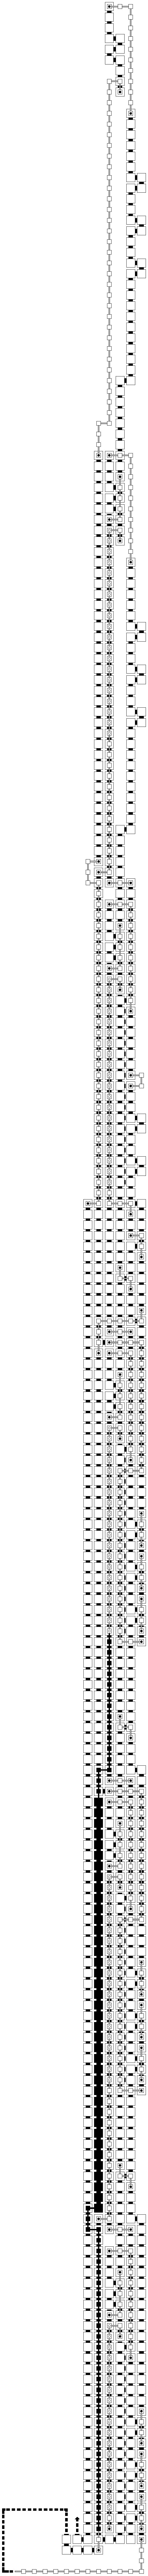
\includegraphics[width=0.45in]{overviews/general/return_path_3_seed_op}}}%
    ~
    \subcaptionbox{Digit 1 - case 2 \label{fig:return_path_1_op_msr}}
    {\makebox[0.24\textwidth][c]{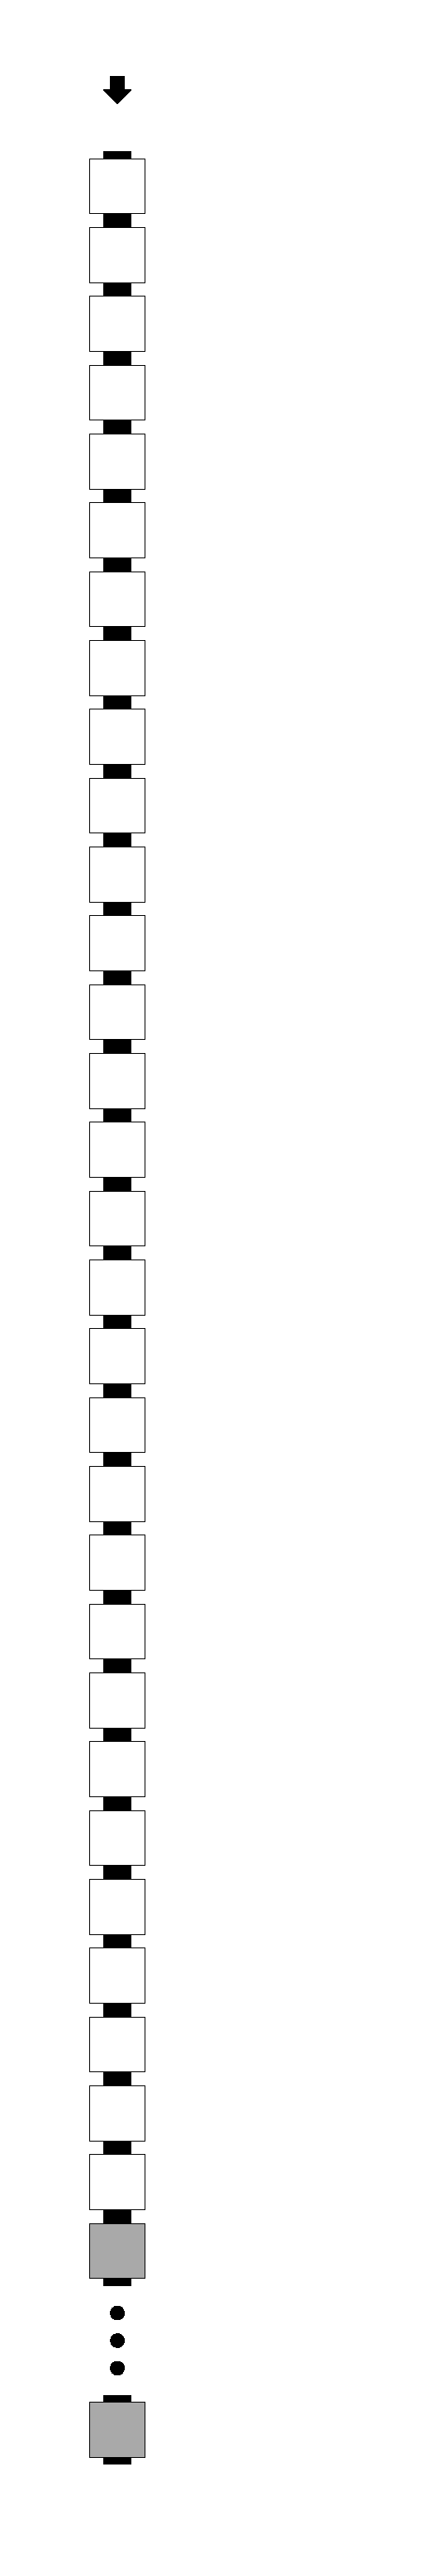
\includegraphics[width=0.45in]{return_path_1_op_msr}}}%
    ~
    \subcaptionbox{Digit 1 - case 2 overview\label{fig:return_path_1_op_msr_overview}}
    {\makebox[0.24\textwidth][c]{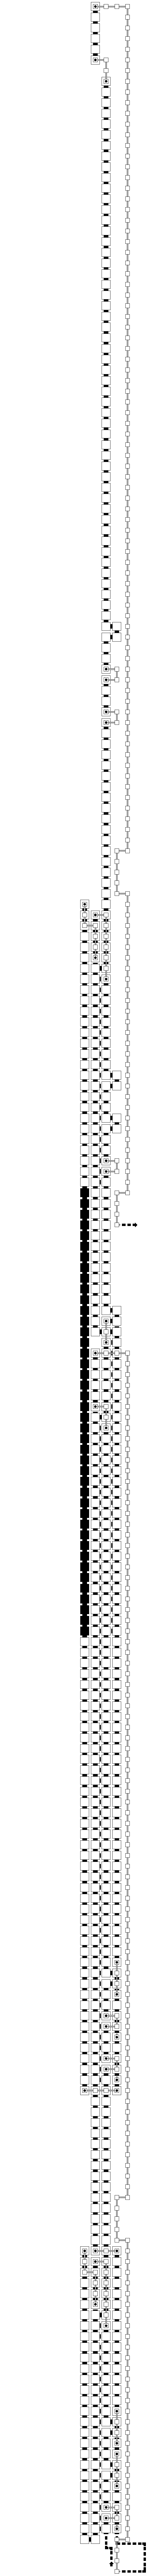
\includegraphics[width=0.45in]{overviews/case2/return_path_1_op_msr}}}%
    ~
    \subcaptionbox{Digit 1 - case 2 (seed) overview (single tile)\label{fig:return_path_1_seed_op_msr_overview}}
    {\makebox[0.24\textwidth][c]{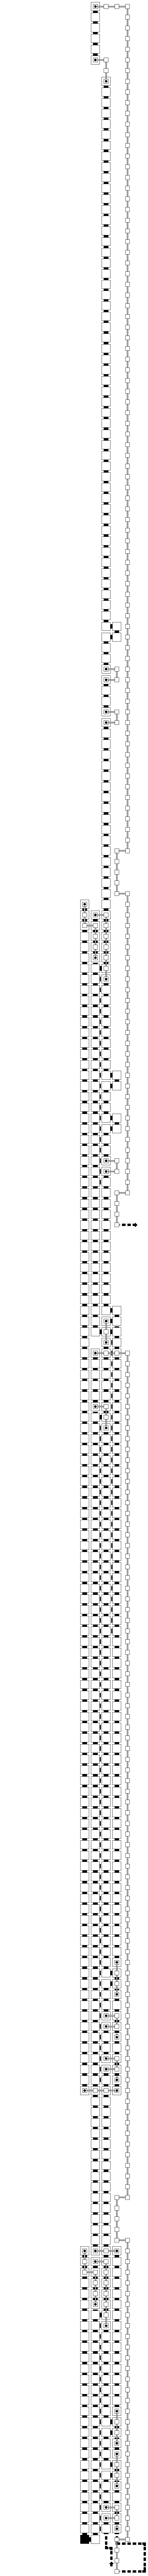
\includegraphics[width=0.45in]{overviews/case2/return_path_1_seed_op_msr}}}%
    ~
\end{figure}

\begin{figure}[H]\ContinuedFloat
    \subcaptionbox{Digit 1 - case 1, Digit 2 case 2\label{fig:return_path_1-or-2_op_msr_msd}}
    {\makebox[0.24\textwidth][c]{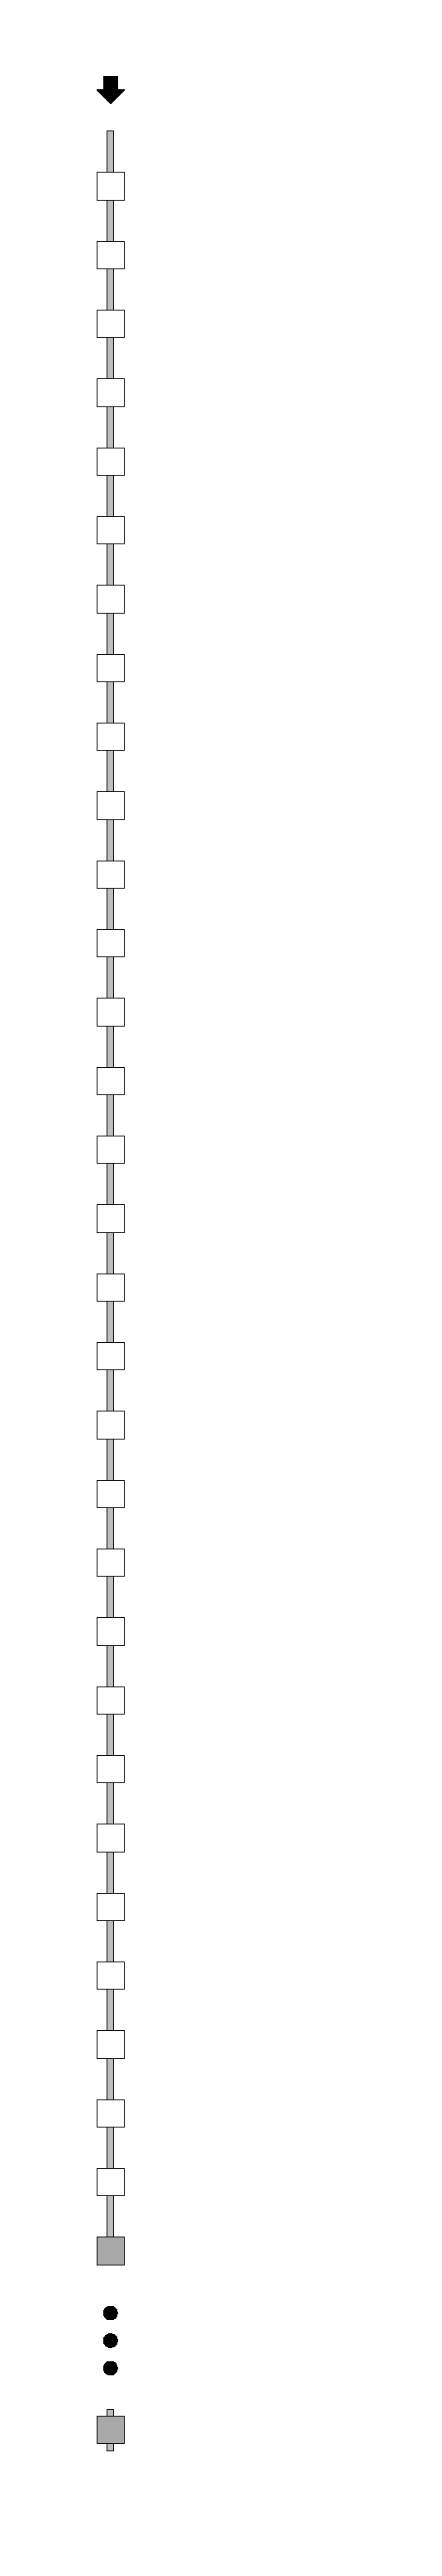
\includegraphics[width=0.45in]{return_path_1-or-2_op_msr_msd}}}%
    ~
    \subcaptionbox{Digit 1 - case 1 overview\label{fig:return_path_1_op_msr_msd_overview}}
    {\makebox[0.24\textwidth][c]{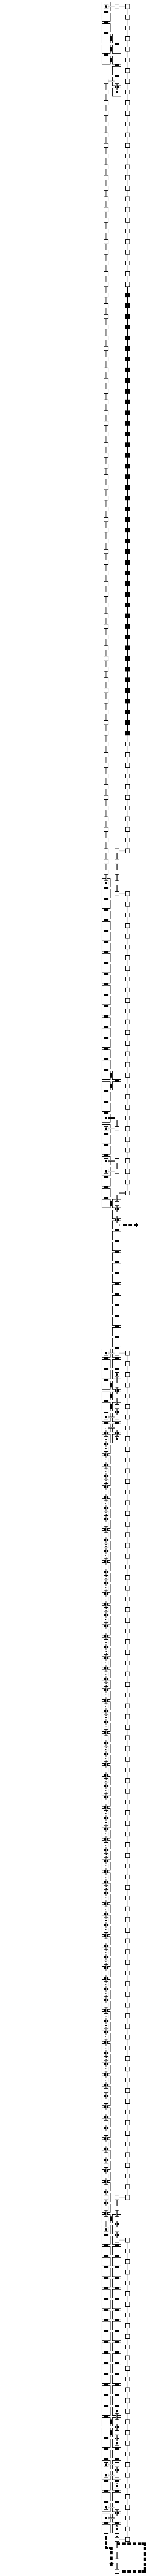
\includegraphics[width=0.45in]{overviews/case1/return_path_1_op_msr_msd}}}%
    ~
    \subcaptionbox{Digit 1 - case 1 (seed) overview\label{fig:return_path_1_seed_op_msr_msd_overview}}
    {\makebox[0.24\textwidth][c]{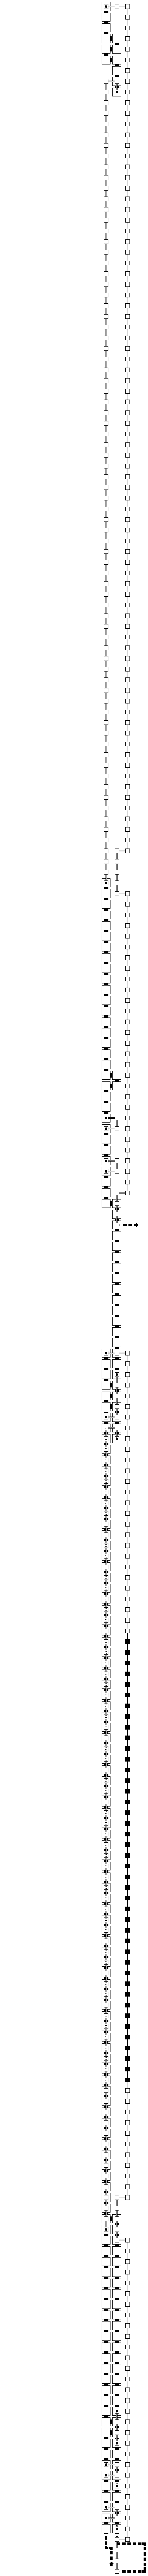
\includegraphics[width=0.45in]{overviews/case1/return_path_1_seed_op_msr_msd}}}%
    ~
    \subcaptionbox{Digit 2 - case 2 overview\label{fig:return_path_2_op_msr_msd_overview}}
    {\makebox[0.24\textwidth][c]{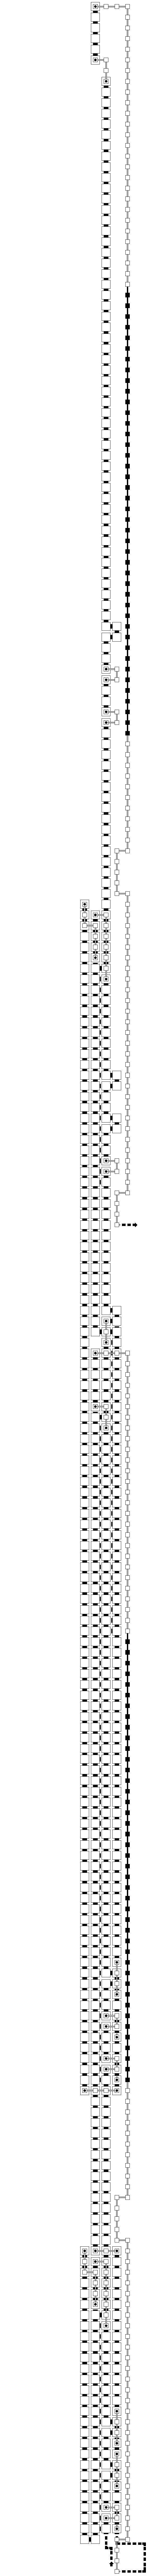
\includegraphics[width=0.45in]{overviews/case2/return_path_2_op_msr_msd}}}%
    ~
    \caption{\label{fig:return_path_gadgets} The {\tt Return\_Path} gadgets.}
\end{figure}

